\documentclass[a4paper,12pt]{article} % тип документа
\usepackage[margin=1in]{geometry} % Поля

%  Русский язык
\usepackage[warn]{mathtext}
\usepackage[T2A]{fontenc}			% кодировка
\usepackage[utf8]{inputenc}			% кодировка исходного текста
\usepackage[english,russian]{babel}	% локализация и переносы
% Математика
\usepackage{amsmath,amsfonts,amssymb,amsthm,mathtools} 
\usepackage{wasysym}
%%%
\usepackage{graphicx}

\usepackage{tabularx}

\usepackage{gensymb} % знак градуса
\usepackage{enumitem} % изменить список enumerate
\usepackage{placeins} % \FloatBarrier

\renewcommand{\thesection}{\Roman{section}} 
\renewcommand{\thesubsection}{\roman{subsection}}


\begin{document}

\newcolumntype{Y}{>{\centering\arraybackslash}X} %new tabularx


%титул
\hrule 	
\medskip
\begin{raggedright}
{\large \textbf{Отчёт по работе 5.10.1}}
\\
\medskip
{\Large Электронный парамагнитный резонанс} 
\\
\medskip
{\large Карташов Констанин, Борток Данил Б04-005}
\medskip
\hrule
\medskip
\end{raggedright}


\section{Анотация}

\paragraph{Цель работы:} 
Исследования электронного парамагнитного резонанса (ЭПР) в молекуле дифенилпикрилгидразила (ДФПГ), определение $g$-фактор электрона, измерение ширины линий ЭПР.



\medskip\hrule\medskip

\section{Теоретическая часть}

\subsection{Теоретическая справка}

\paragraph{}В методе ЭПР изучается резонансное поглощение переменного электромагнитного поля в образце в зависимости от контролируемых экспериментатором внешних условий: постоянного магнитного поля, частоты колебаний переменного поля, температуры и так далее.

\paragraph{}Простейшей моделью для рассмотрения ЭПР является система из невзаимодействующих частиц со спином $S = 1/2$, помещённая во внешнее магнитное поле. В отсутствие магнитного поля энергии состояний с проекцией спина $S_Z = \pm 1/2$ совпадают. Из-за эффекта Зеемана энергии состояний с различными проекциями спина начинают различаться. Если направить на нашу систему поток излучения с энергией, равной разнице энергий этих состояний 

\begin{equation}
\label{e:2}
h \nu = g\mu_B B,
\end{equation} 

\noindent то станут возможны индуцированные переходы между состояниями. Эти переходы происходят с поглощением или испусканием фотона в зависимости от того, в каком из состояний была система до взаимодействия с излучением. В отличие от оптических переходов между электронными уровнями энергии в атоме, типичная частота переменного поля в ЭПР эксперименте составляет порядка 10 ГГц (а в нашем лабораторном эксперименте около 100 МГц), что соответствует энергии фотона менее 1К. Поэтому, за исключением очень низких температур, заселённость обоих спиновых подуровней с $S_Z = \pm 1/2$ близка. В состоянии теплового равновесия нижний энергетический уровень более заселён, поэтому наблюдается поглощение электромагнитного излучения.

\paragraph{}В «классическом» подходе рассматривается прецессия магнитного момента во внешнем поле при отклонении магнитного момента от равновесия. Классический магнитный диполь стремится выровняться вдоль силовых линий магнитного поля, при отклонении от равновесия возникает возвращающий механический момент $\mathbf{T} = \mathbf{M}\times \mathbf{B}$. Так как магнитный и механический момент иона связаны друг с другом гиромагнитным отношением $\gamma$ как $\mathbf{M}=\gamma \mathbf{J}$ , где $\mathbf{J}$ - это полный момент импульса, то с учётом уравнения динамики
$\frac{d}{dt}\mathbf{J} = \mathbf{T}$, получим уравнение прецессии магнитного момента:

\[
\dfrac{d}{dt}\mathbf{M} = \gamma \mathbf{M} \times \mathbf{B}.
\]
 
\paragraph{}Аналогично с известной задачей о прецессии гироскопа можно заметить, что при отклонении магнитного момента от направления магнитного поля возникает незатухающая прецессия вокруг направления поля с угловой скоростью $\boldsymbol{\Omega} = -\gamma \mathbf{B}$, частота этой прецессии $\Omega_L = \gamma B$ называется ларморовской. При совпадении частоты переменного поля, перпендикулярного основному, с ларморовской частотой возможно возникновение резонансного поглощения.

\subsection{Устройство экспериментальной установки}


\begin{figure}[h]
\centering
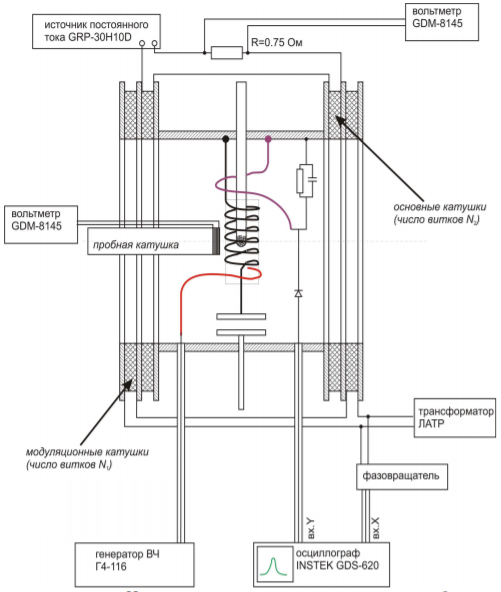
\includegraphics[width=0.7\textwidth]{setup.png}
\caption{Схема экспериментальной установки}
\label{fig:setup}
\end{figure}

\paragraph{} Схема установки представлена на рис. \ref{fig:setup}. Образец (порошок ДФПГ) в стеклянной ампуле помещается внутрь катушки индуктивности, входящей в состав колебательного контура. Входящий в состав контура конденсатор состоит из двух пластин, разделённых воздушным зазором, одна из пластин может перемещаться поворотом штока. Колебания в контуре возбуждаются антенной, соединённой с генератором высокой частоты (ВЧ) Г4-116. Амплитуда колебаний поля в катушке индуктивности измеряется по наводимой в петле связи ЭДС индукции. Высокочастотные колебания ЭДС индукции в приёмном контуре детектируются диодом, измеряемая при помощи осциллографа низкочастотная огибающая этого сигнала пропорциональна квадрату амплитуды колебаний поля в катушке.

\paragraph{}Постоянное магнитное поле создаётся пропусканием тока от источника постоянного тока через основные катушки. При этом при помощи вольтметра измеряется падение напряжения на резисторе в цепи основных катушек. Переменное поле небольшой амплитуды создаётся подачей на модуляционные катушки напряжения с регулируемого трансформатора ЛАТР. Для измерения амплитуды колебаний переменного поля используется пробная катушка известной геометрии, подключённая к вольтметру. Пусть поток через неё $\Phi_{\text{проб}}$, тогда ЭДС индукции:

\[
\mathcal{E} = - \dfrac{d\Phi_{\text{проб}}}{dt}.
\]

Если $I_{\text{осн}}$ -- ток через основную катушку, а $M$ -- взаимная индуктивность основной и пробной катушек, то:

\[
\Phi_{\text{проб}} = M I_{\text{осн}}.
\]

Тогда амплитудное значение ЭДС индукции:

\[
\mathcal{E}_{\text{амп}} = - \dfrac{dM I_{\text{осн}}}{dt} = M \omega I_{\text{амп}}.
\]

Учитывая, что $I_{\text{амп}} = \sqrt{2} I_{\text{действ}}=\frac{V_r}{r}$, где $V_R$, $R$ -- напряжение на резисторе с сопротивлением $R$ в цепи основных катушек, а также $\mathcal{E}_{\text{амп}} = \sqrt{2}\mathcal{E}_{\text{ср}}$, получим:

\[
\mathcal{E}_{\text{ср}} = M \omega \dfrac{V_R}{R} = k V_R.
\]

Тогда, зная, что:
\[
\Phi_{\text{проб}} = B_0 N_{\text{проб}} \dfrac{\pi d_{\text{проб}}^2}{4} =  \dfrac{MU_R}{R} = \dfrac{k U}{\omega},
\]

\noindent где $U$ -- напряжение на $R$ в резонансе, получим:

\begin{equation}
\label{e:1}
B_0 = \dfrac{4k U}{\pi \omega d^2_{\text{проб}} N_{\text{проб}}}.
\end{equation}

Характеристики катушек: пробная катушка $N_{\text{проб}} = 45$, $d_{\text{проб}} = 14.5\pm 0.1~\text{мм}$, основная катушка $N_{\text{осн}} = 4500$, $d_{\text{осн}} = 0.29\pm 0.01~\text{м}$,  модулирующая катушка $N_{\text{мод}} = 1500$, $d_{\text{мод}} = 0.23\pm 0.01~\text{м}$.


\medskip\hrule\medskip

\section{Экспериментальная часть}

\subsection{Настройка ВЧ генератора.}

\paragraph{}Генератор настраиваем на частоту колебательного контура: в режиме амплитудной модуляции 10\% устанавливаем подстройкой частоты генератора добиваемся максимальной амплитуды сигнала на экране осциллографа. Частоту определяем по шкале генератора, $f_0 = 125.5 \pm 0.2~\text{МГц}$ (погрешность всех измерений частот -- цена деления грубой шкалы $\sigma_f = 0.2~\text{МГц}$). 

\subsection{Наблюдение сигнала резонансного поглощения.}
\paragraph{}Подключим основные катушки к источнику постоянного тока, а модуляционные катушки к трансформатору ЛАТР. ВЧ-генератор переведём в режим непрерывной генерации, на канале осциллографа, подключённому к детектору, установим максимальную чувствительность. Подадим на модуляционные катушки напряжение $\sim 50~\text{В}$, и, плавно увеличивая постоянное напряжение на основных катушках, добиваемся возникновения на экране резонансного поглощения. Добьёмся того, чтобы наблюдаемые пики были эквидистантными. Зафиксируем напряжение на резисторе $R$.

\subsection*{Точная настройка резонансного поля и определение ширины линии.}
\paragraph{}Для более точной настройки и определения ширины линии резонансного поглощения удобно подать на X-канал осциллографа напряжение, прикладываемое к модуляционным катушкам и наблюдать сигнал в XY-режиме. Фактически при этом на экране наблюдается зависимость поглощения в образце от приложенного переменного поля. Наблюдаемая картина симметрична относительно средней вертикальной оси. Из-за набегающей в электрической схеме расфазировки напряжений на экране наблюдаются два пика, соответствующие прохождению резонансного поглощения на растущем и падающем полупериодах модулирующего напряжения, поэтому пики совмещаем подстройкой фазовращателя.

\paragraph{}Для определения ширины линии ЭПР определим по экрану осциллографа полный размах
модулирующего поля $A_{\text{полн}}$ и полную ширину кривой резонансного
поглощения на полувысоте $A_{\text{1/2}}$ . Не изменяя настроек, возьмём пробную катушку и внесём её внутрь соленоида максимально близко к образцу. Переменное поле модуляционных катушек наводит в пробной катушке ЭДС индукции $\mathcal{E}$, по которой можно определить величину поля. ЭДС индукции: $\mathcal{E}_i = 0.86\pm 0.04~\text{мВ}$ (погрешность измерения вольтметра 0.03\% + 4 единицы последнего знака). Размах и ширина кривой резонансного поглощения $A_{\text{полн}} = 6.2 \pm 0.2~\text{дел}$, $A_{\text{1/2}} = 0.8 \pm 0.2~\text{дел}$ (погрешность -- размер минимального деления осцилографа). Тогда амплитуда модулюрующего поля:

\[
B_{\text{мод}} = \dfrac{2\sqrt{2}\mathcal{E}_i}{\pi^2 d_{\text{проб}}^2 N_{\text{проб}}\nu} = 5.2 \pm 0.3~\text{Гс},
\]

\noindent где погрешность рассчитана по формуле:

\[
\sigma_{B_{\text{мод}}}=\sqrt{\left(\dfrac{\partial B_{\text{мод}}}{\partial \mathcal{E}_i} \right)^2 \sigma^2_{\mathcal{E}i} + \left(\dfrac{\partial B_{\text{мод}}}{\partial d_{\text{проб}}} \right)^2 \sigma^2_{d_{\text{проб}}}},
\]

\noindent и $\nu = 50~\text{Гц}$ -- частота модулирующего напряжения. Полуширину на полувысоте линии резонансного поглощения посчитаем по формуле:

\[
\Delta B = \dfrac{A_{1/2}}{A_{\text{полн}}} B_{\text{мод}} = 0.67 \pm 0.04~\text{Гс},
\]

\noindent где погрешность рассчитана по формуле:
\[\sigma_{\Delta B} = \sqrt{ \left(\dfrac{\partial \Delta B}{\partial A_{\text{полн}}} \right)^2 \sigma^2_{A_{\text{полн}}} +  \left(\dfrac{\partial \Delta B}{\partial A_{\text{1/2}}} \right)^2 \sigma^2_{A_{\text{1/2}}} + \left(\dfrac{\partial \Delta B}{\partial B_{\text{мод}}} \right)^2 \sigma^2_{B_{\text{мод}}} }.\]

\subsection{Калибровка поля электромагнита и определение g-фактора.}

\paragraph{}Для определения поля резонансного поглощения найдём связь между падением напряжения на резисторе в цепи основной катушки и магнитным полем. Для этого подадим в основные катушки переменный ток и измеряем при помощи пробной катушки
ЭДС индукции.

\paragraph{}Переключим основные катушки на ЛАТР, переведём вольтметр, измеряющий
падение напряжения на резисторе $\mathcal{E}_0$ в цепи основных катушек, в режим измерений на
переменном токе, установим ток через катушки, близкий к значению тока при наблюдении резонансного поглощения, измерим в этих условиях ЭДС индукции в пробных катушках. Получаем $\mathcal{E}_0 = 10.3 \pm 0.1$ мВ.

\paragraph{}Теперь мы можем посчитать индукцию основного магнитного поля по \eqref{e:1}:

\[
B_0 = \dfrac{2 \sqrt{2} \mathcal{E}_0}{\pi^2 d_{\text{проб}}^2 N_{\text{проб}}} = 62 \pm 1~\text{Гс},
\]

\paragraph{} Тогда $g$-фактор электрона будет по формуле \eqref{e:2} равен:

\[
g = \dfrac{hf_0}{\mu_B B_0} = 1.4 \pm 0.1,
\]

\noindent погрешность считалась по формуле:
\[
\sigma_g = \sqrt{ \left( \dfrac{\partial g}{\partial f_0}\right)^2 \sigma_{f_0}^2 + \left( \dfrac{\partial g}{\partial B_0}\right)^2 \sigma_{B_0}^2}.
\]

\paragraph{} Истинное значение $g$-фактора электрона $g = 2.0036$.
\medskip\hrule\medskip

\section{Выводы}

\paragraph{}В данной работе был исследован ЭПР в молекуле ДФПГ, определяется $g$-фактор электрона $g = 1.4 \pm 0.1$, а также измерена ширина линий ЭПР $\Delta B = 0.67 \pm 0.04~\text{Гс}$. Большое различие между измеренным и действительным $g$-фактор может быть устранение путём измерение напряжённости магнитного поля внутри катушки с разных сторон для вычета неоднородности магнитного поля, и при различных напряжениях на катушке.


\medskip\hrule\medskip

\end{document}
